% Chapter 3: Analysis and Design - Revised for Intelligent Content Management Platform
\chapter{Analysis and Design}

This chapter presents the comprehensive technical architecture, requirements specification, and design models for VocalizeWeb. The analysis encompasses functional capabilities for multi-modal interaction and RAG-based content retrieval, alongside non-functional requirements for accuracy, scalability, and performance. Design artifacts provide visual representations of the conversational AI system.

\section{Functional Requirements}

Functional requirements define the specific behaviors and transformations that VocalizeWeb must execute, organized by subsystem.

\subsection{Multi-Modal Interaction Requirements}

\subsubsection{Text-Based Chatbot}

\begin{enumerate}[leftmargin=*]
    \item FR-TEXT-01: The system shall provide a text input interface embedded as a floating widget.
    \item FR-TEXT-02: The system shall process natural language text queries and generate contextual responses.
    \item FR-TEXT-03: The system shall maintain conversational context across multiple exchanges within a session.
    \item FR-TEXT-04: The system shall display typing indicators during response generation.
    \item FR-TEXT-05: The system shall support conversation transcript viewing and export.
\end{enumerate}

\subsubsection{Voice-to-Voice Assistant}

\begin{enumerate}[leftmargin=*]
    \item FR-VOICE-01: The system shall capture audio input from the user's browser microphone.
    \item FR-VOICE-02: The system shall convert spoken input to text using Whisper Turbo STT service.
    \item FR-VOICE-03: The system shall support voice activity detection to distinguish speech from silence.
    \item FR-VOICE-04: The system shall convert AI-generated text responses to speech using OpenAI TTS.
    \item FR-VOICE-05: The system shall stream synthesized audio back to the user's browser.
    \item FR-VOICE-06: The system shall support voice cancellation, allowing users to interrupt responses.
    \item FR-VOICE-07: The system shall provide visual indicators for listening, processing, and speaking states.
\end{enumerate}

\subsubsection{Modality Configuration}

\begin{enumerate}[leftmargin=*]
    \item FR-MODE-01: The system shall support client configuration of enabled modalities (text, voice, or both).
    \item FR-MODE-02: The widget shall adapt its interface based on configured modalities.
    \item FR-MODE-03: The system shall validate modality availability before enabling voice features.
\end{enumerate}

\subsection{Content Management Requirements}

\begin{enumerate}[leftmargin=*]
    \item FR-CONTENT-01: The system shall support document upload in PDF, DOCX, and TXT formats.
    \item FR-CONTENT-02: The system shall extract text content from uploaded documents.
    \item FR-CONTENT-03: The system shall scrape content from specified website URLs.
    \item FR-CONTENT-04: The system shall chunk extracted text with configurable size and overlap.
    \item FR-CONTENT-05: The system shall generate vector embeddings for text chunks.
    \item FR-CONTENT-06: The system shall store embeddings in vector database (Weaviate/Redis).
    \item FR-CONTENT-07: The system shall maintain content-to-source mapping for citation.
    \item FR-CONTENT-08: The system shall support manual content entry through administrative interface.
    \item FR-CONTENT-09: The system shall provide API endpoints for programmatic content submission.
    \item FR-CONTENT-10: The system shall allow clients to update content by re-uploading or re-scraping.
\end{enumerate}

\subsection{SaaS Platform Requirements}

\subsubsection{Client Management}

\begin{enumerate}[leftmargin=*]
    \item FR-CLIENT-01: The system shall support client registration with organization details.
    \item FR-CLIENT-02: The system shall assign unique API keys per client deployment.
    \item FR-CLIENT-03: The system shall enforce API key authentication on all requests.
    \item FR-CLIENT-04: The system shall support API key regeneration for security purposes.
\end{enumerate}

\subsubsection{Feature Toggle Management}

\begin{enumerate}[leftmargin=*]
    \item FR-TOGGLE-01: The system shall provide configurable feature toggles per client.
    \item FR-TOGGLE-02: The system shall support modality toggle (text/voice/both).
    \item FR-TOGGLE-03: The system shall support auto-scraping toggle (enabled/disabled).
    \item FR-TOGGLE-04: The system shall support update approval mode toggle (manual/automatic).
    \item FR-TOGGLE-05: The system shall apply toggle changes without system restart.
\end{enumerate}

\subsubsection{Session and Conversation Management}

\begin{enumerate}[leftmargin=*]
    \item FR-SESSION-01: The system shall generate unique session identifiers for each user interaction.
    \item FR-SESSION-02: The system shall terminate sessions after configurable inactivity timeout.
    \item FR-SESSION-03: The system shall preserve conversation histories per session.
    \item FR-SESSION-04: The system shall support conversation export in JSON and CSV formats.
\end{enumerate}

\section{Non-Functional Requirements}

\subsection{Performance Requirements}

\begin{enumerate}[leftmargin=*]
    \item NFR-PERF-01: The system shall achieve end-to-end text query response times under 3 seconds.
    \item NFR-PERF-02: The system shall achieve end-to-end voice-to-voice response times under 5 seconds.
    \item NFR-PERF-03: The system shall complete web scraping within 60 seconds per page.
\end{enumerate}

\subsection{Accuracy Requirements}

\begin{enumerate}[leftmargin=*]
    \item NFR-ACC-01: The system shall achieve RAG retrieval relevance exceeding 90\%.
    \item NFR-ACC-02: The system shall achieve speech recognition accuracy suitable for conversational AI.
\end{enumerate}

\subsection{Scalability Requirements}

\begin{enumerate}[leftmargin=*]
    \item NFR-SCALE-01: The system shall support 100+ client websites concurrently.
    \item NFR-SCALE-02: The system shall support 1000+ concurrent user sessions.
    \item NFR-SCALE-03: The system shall support knowledge bases up to 100,000 content items per client.
    \item NFR-SCALE-04: The architecture shall support horizontal scaling via additional instances.
\end{enumerate}

\subsection{Reliability Requirements}

\begin{enumerate}[leftmargin=*]
    \item NFR-REL-01: The system shall implement graceful degradation when external AI services fail.
    \item NFR-REL-02: The system shall retry failed API calls with exponential backoff (max 3 retries).
    \item NFR-REL-03: The system shall maintain update operation atomicity (all-or-nothing).
    \item NFR-REL-04: The system shall log all errors with sufficient detail for debugging.
\end{enumerate}

\subsection{Security Requirements}

\begin{enumerate}[leftmargin=*]
    \item NFR-SEC-01: The system shall transmit all data over HTTPS/TLS 1.2+.
    \item NFR-SEC-02: The system shall validate and sanitize all user inputs.
    \item NFR-SEC-03: The system shall implement rate limiting per API key.
    \item NFR-SEC-04: The system shall enforce data isolation between client tenants.
    \item NFR-SEC-05: The system shall store API keys using secure hashing.
\end{enumerate}

\section{System Models}

\subsection{Data Flow Diagrams}

\subsubsection{Level 0 DFD (Context Diagram)}

Figure~\ref{fig:dfd0} shows the system boundary with external entities. VocalizeWeb interacts with End Users (text/voice queries), Website Owners (configuration and content), and AI Services (STT, LLM, TTS, Embeddings).

\begin{figure}[H]
    \centering
    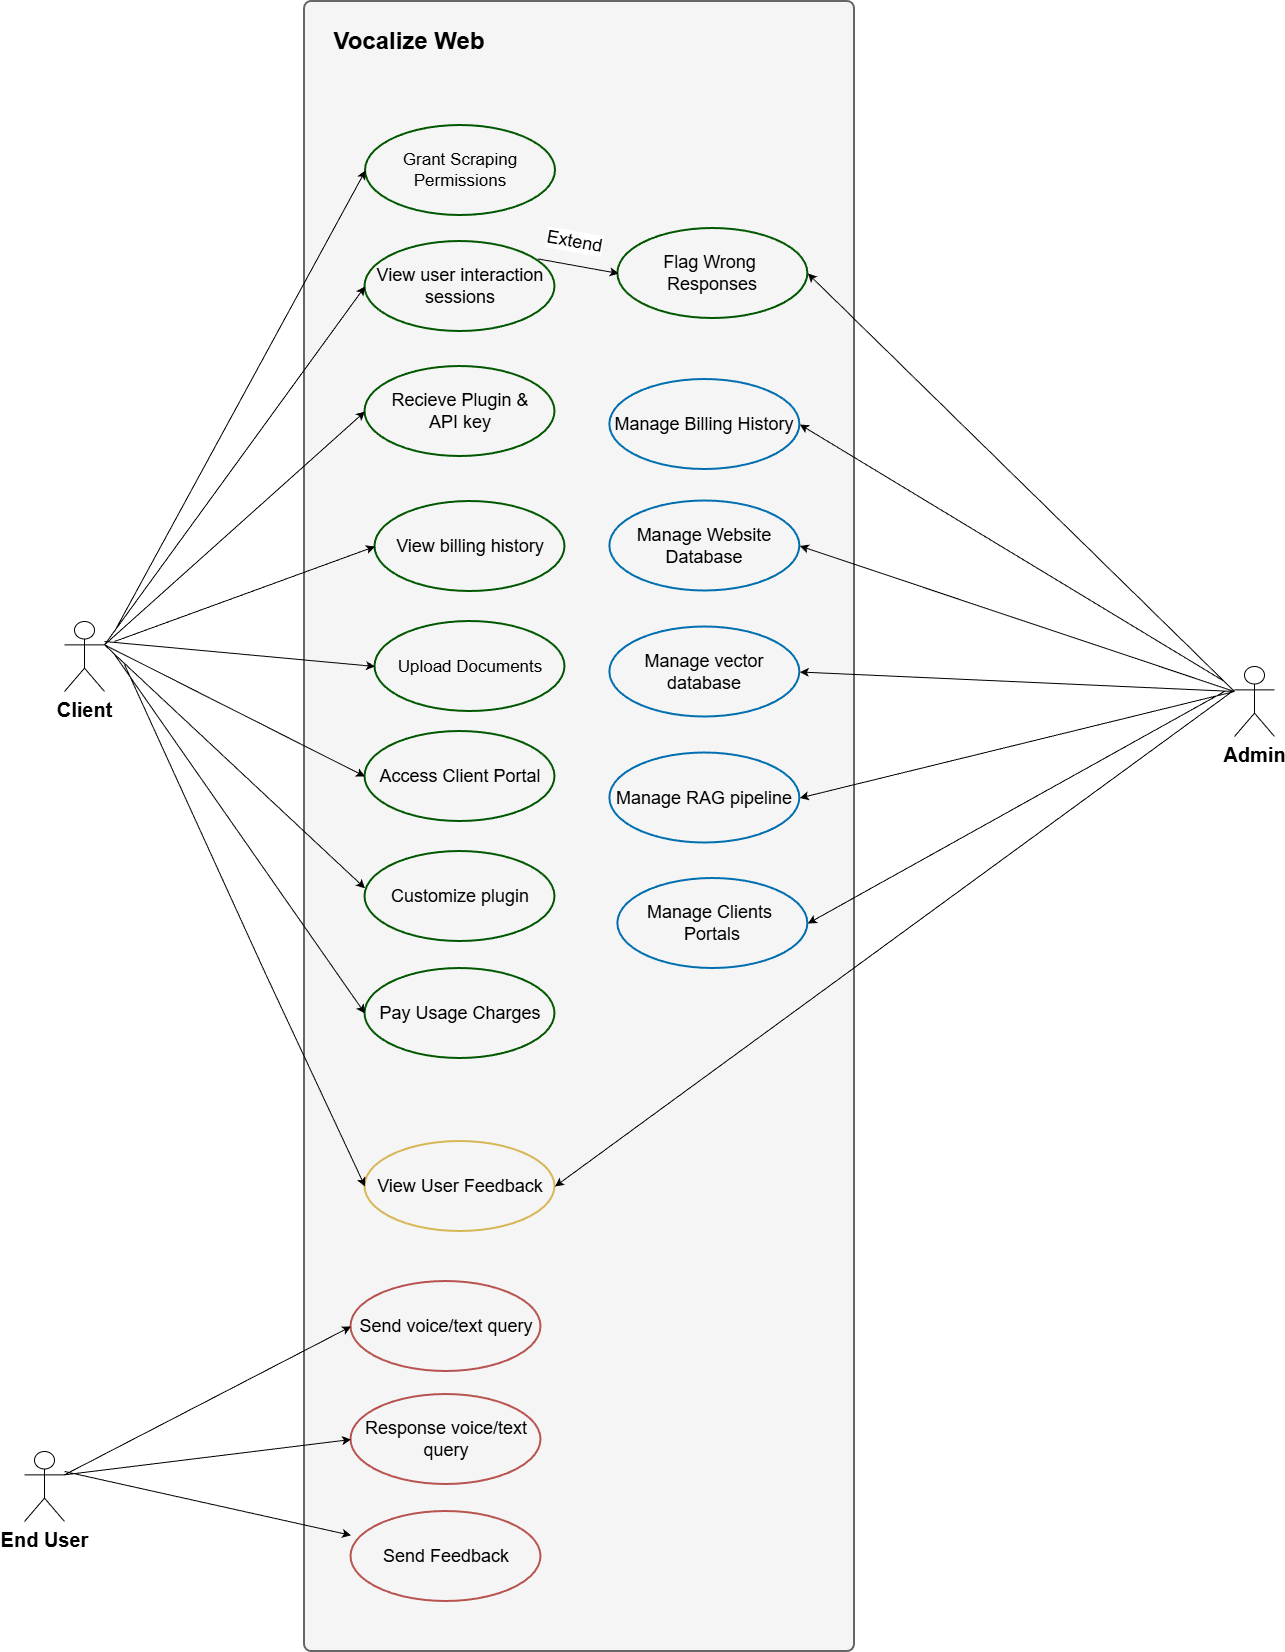
\includegraphics[width=0.95\textwidth]{diagrams/dfd_level_0.png}
    \caption{Level 0 DFD (Context Diagram) - System Boundary View}
    \label{fig:dfd0}
\end{figure}

\subsubsection{Level 1 DFD}

Figure~\ref{fig:dfd1} decomposes the system into major processes: Query Router, Content Ingestion, RAG Pipeline, and Voice Processing. Data stores include Vector DB and SaaS Platform DB.

\begin{figure}[H]
    \centering
    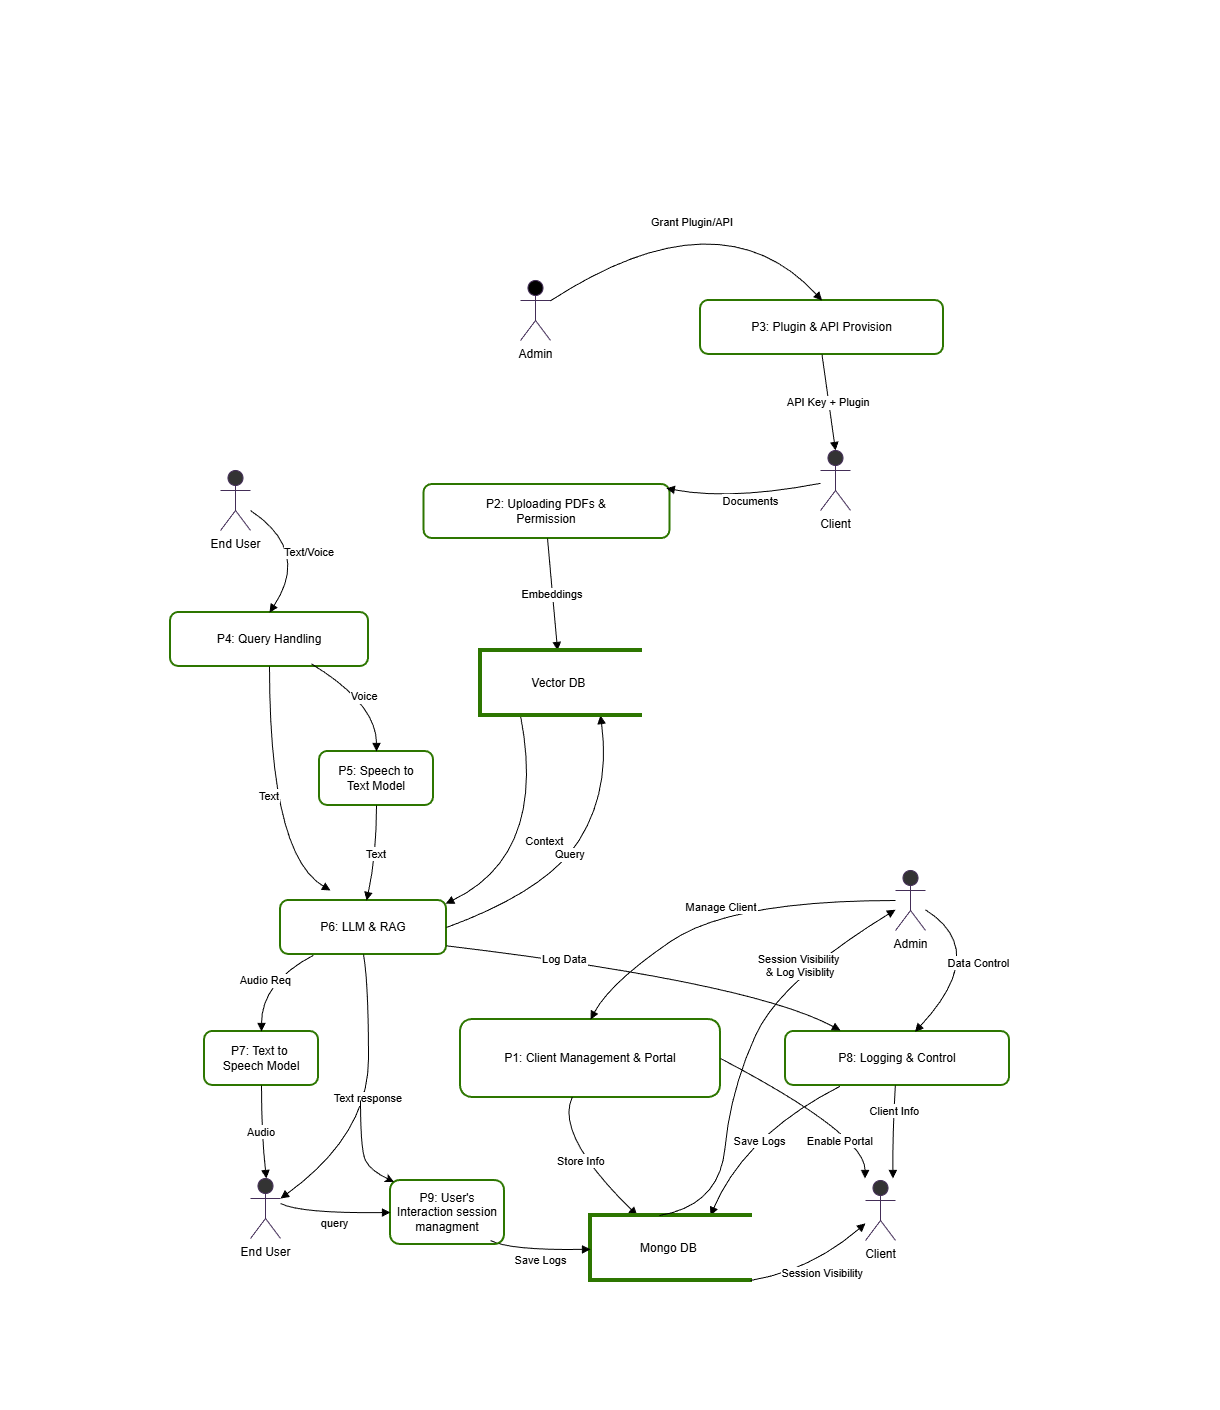
\includegraphics[width=0.85\textwidth]{diagrams/dfd_level1.png}
    \caption{Level 1 DFD - Process Decomposition with Content Types}
    \label{fig:dfd1}
\end{figure}

\subsection{System Architecture Diagram}

Figure~\ref{fig:architecture} presents the high-level system architecture showing the multi-modal frontend, API gateway, processing engines, and multi-database storage layer.

\begin{figure}[H]
    \centering
    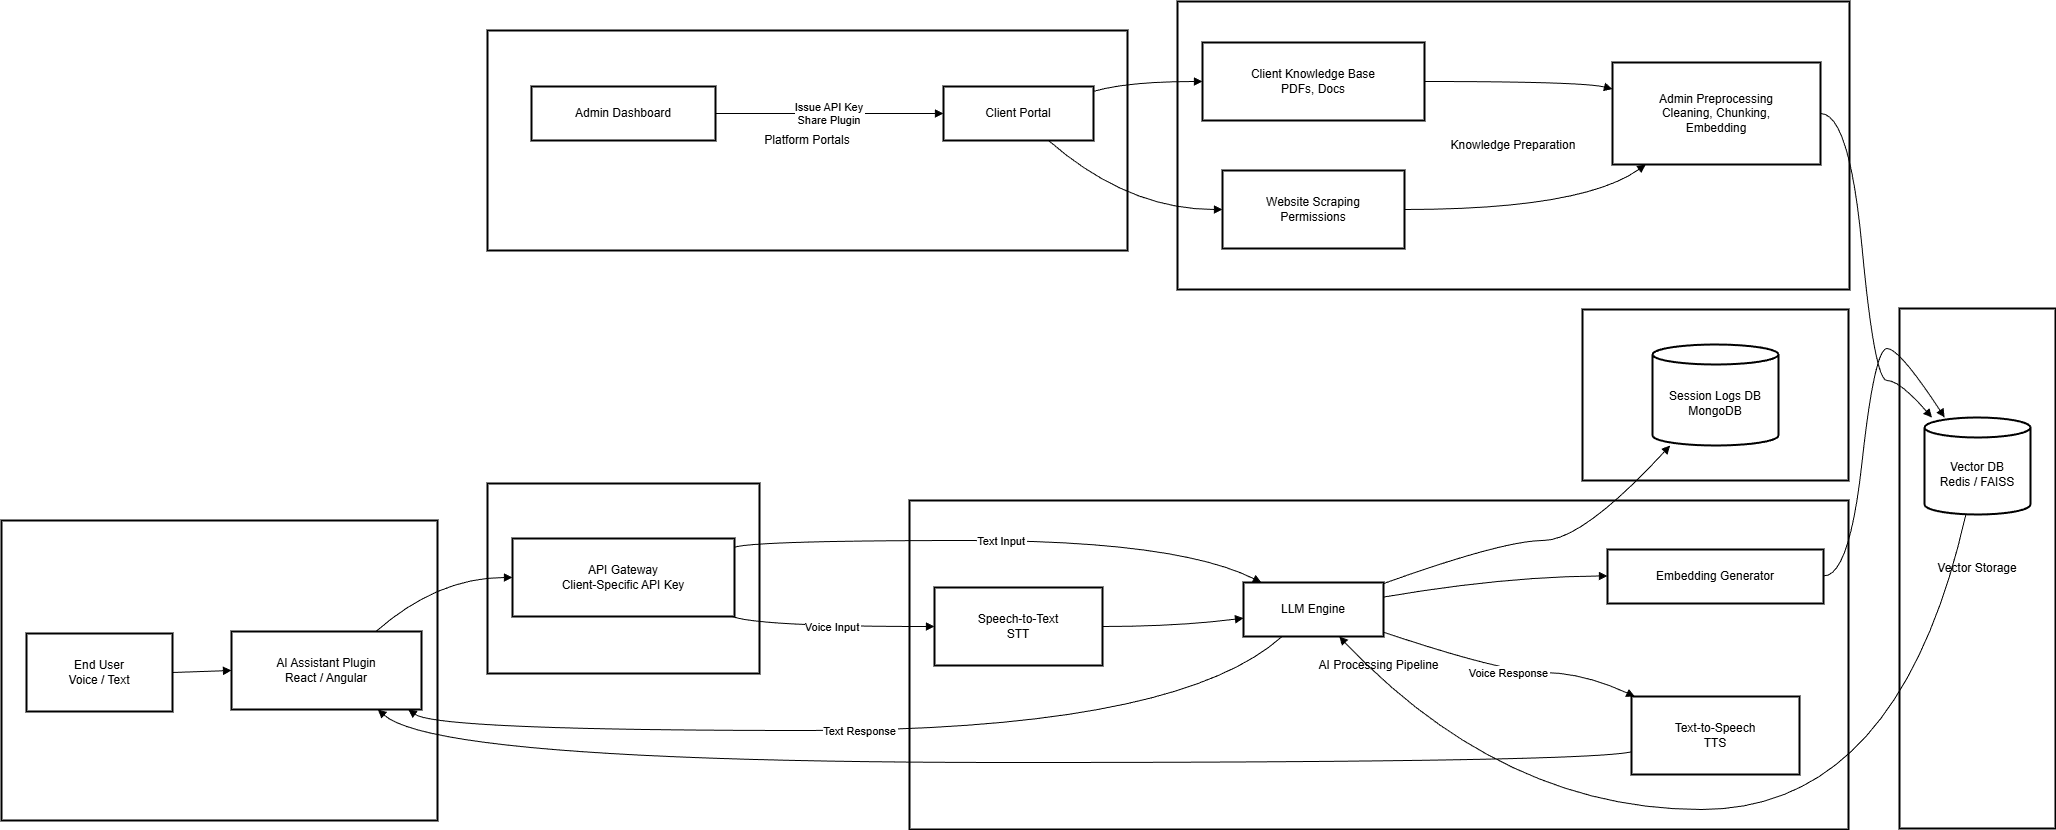
\includegraphics[width=0.95\textwidth]{diagrams/architecture.png}
    \caption{High-Level System Architecture}
    \label{fig:architecture}
\end{figure}

\subsection{Use Case Diagram}

Figure~\ref{fig:usecase} identifies actors (End User, Website Owner, System Admin) and their interactions including multi-modal queries, content management, feature configuration, and DOM synchronization.

\begin{figure}[H]
    \centering
    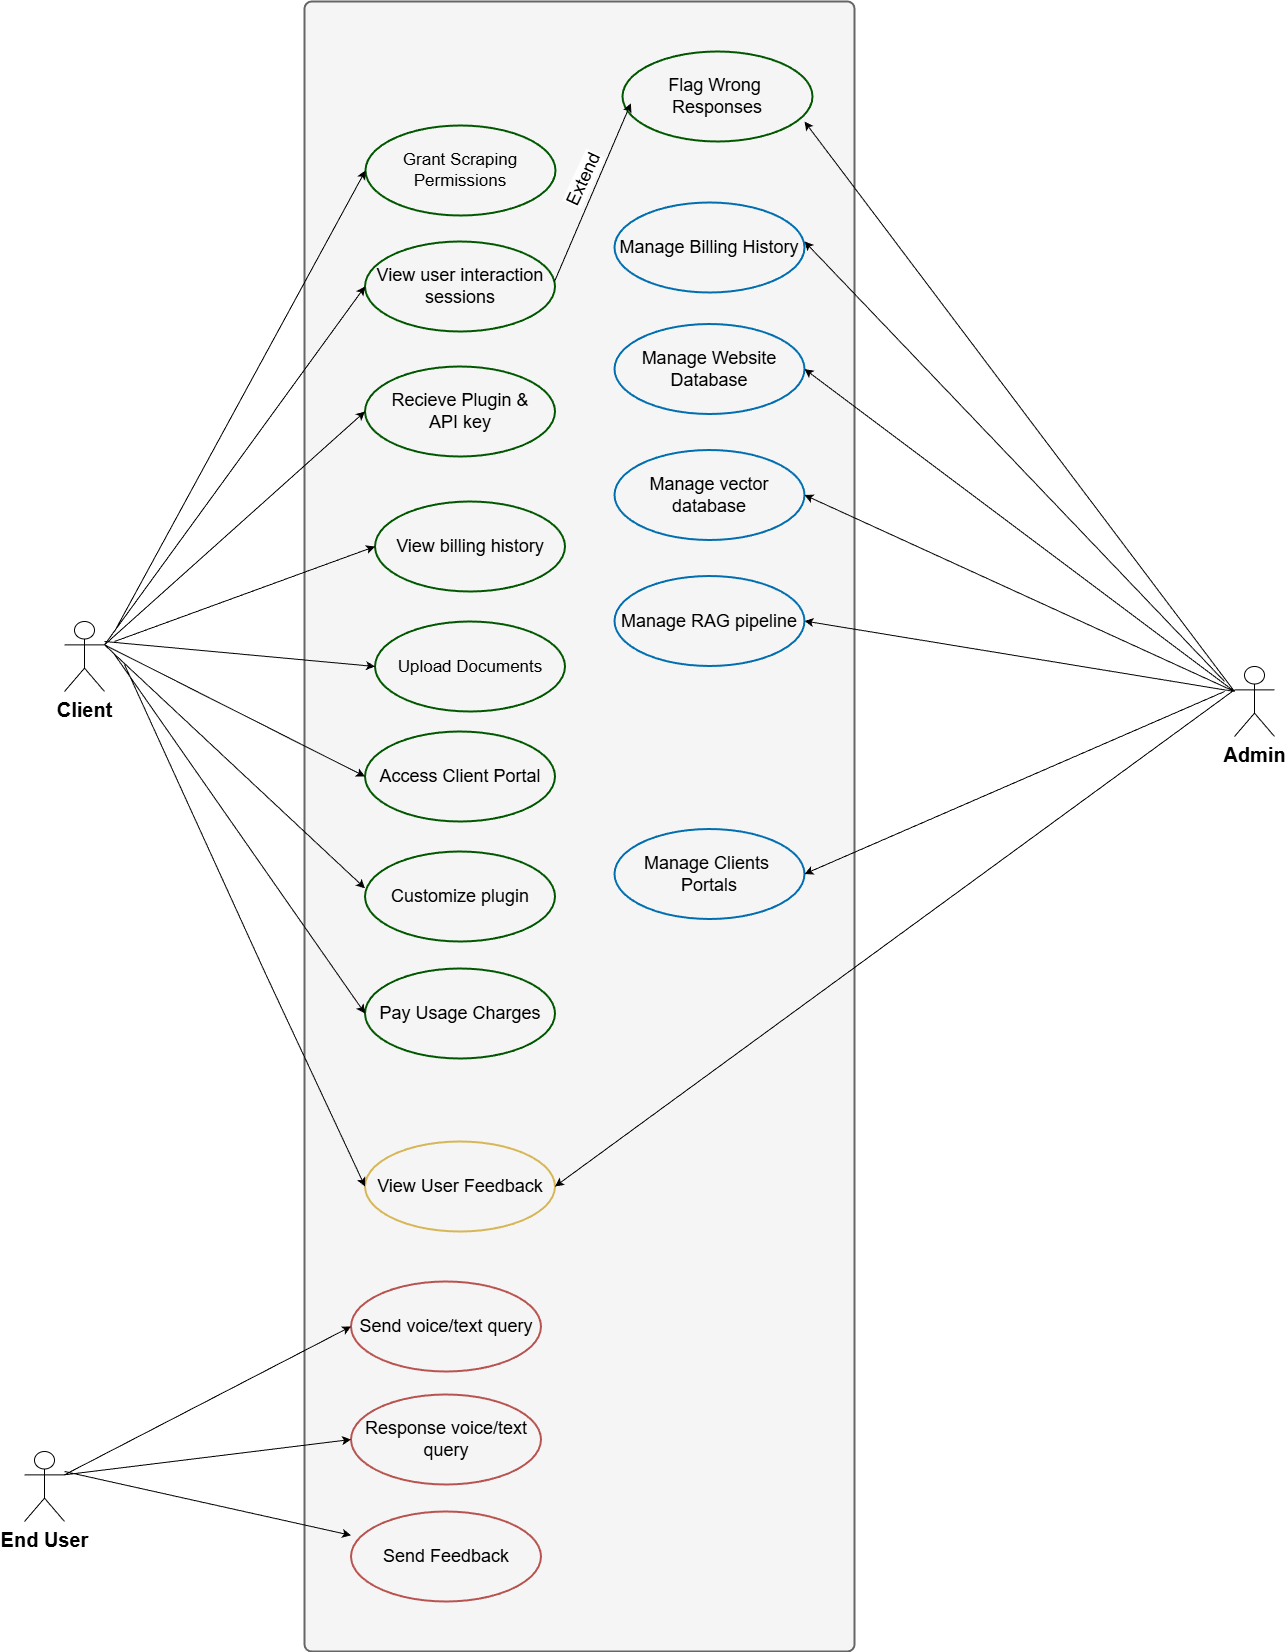
\includegraphics[height=0.75\textheight,keepaspectratio]{diagrams/use_case.png}
    \caption{Use Case Diagram - Actor Interactions}
    \label{fig:usecase}
\end{figure}

\subsection{Entity-Relationship Diagram}

Figure~\ref{fig:erd} models the database schema including Client, KnowledgeBase, ContentItem, Session, Message, and FeatureToggle tables.

\begin{figure}[H]
    \centering
    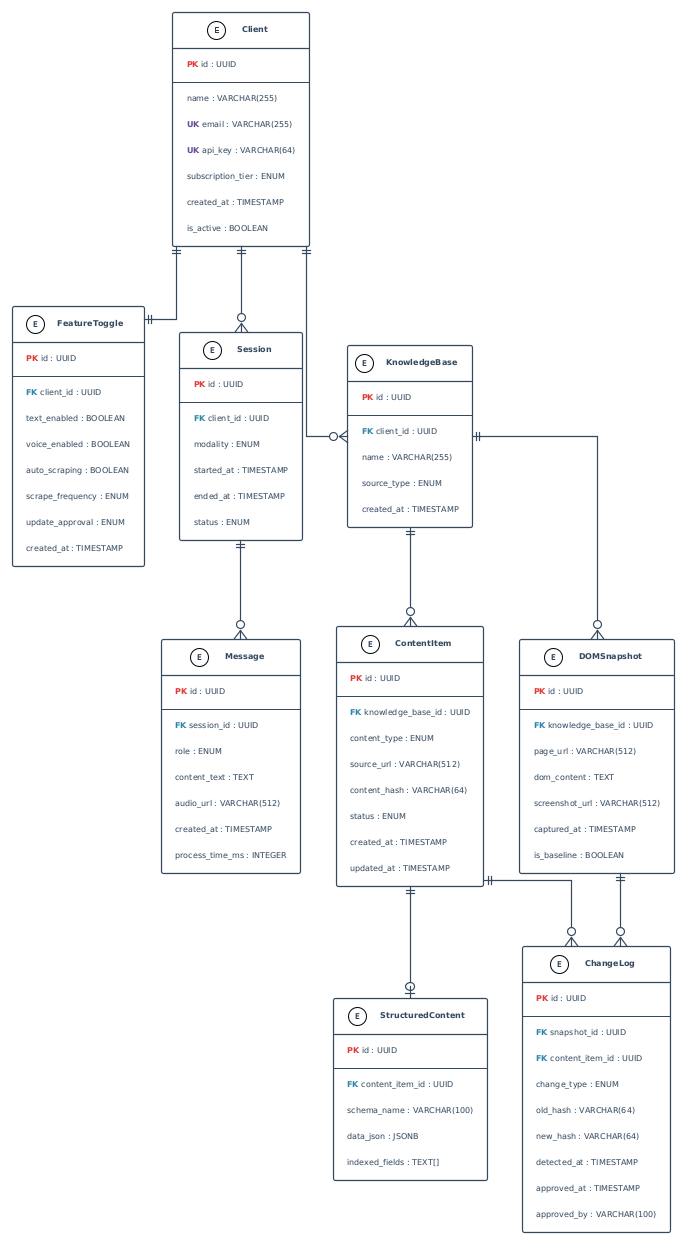
\includegraphics[width=0.85\textwidth]{diagrams/erd.png}
    \caption{Entity-Relationship Diagram - Database Schema}
    \label{fig:erd}
\end{figure}

\subsection{Sequence Diagrams}

\subsubsection{Multi-Modal Query Processing}

Figure~\ref{fig:seq_query} shows the interaction flow for both text and voice queries, including content retrieval from the vector database.

\begin{figure}[H]
    \centering
    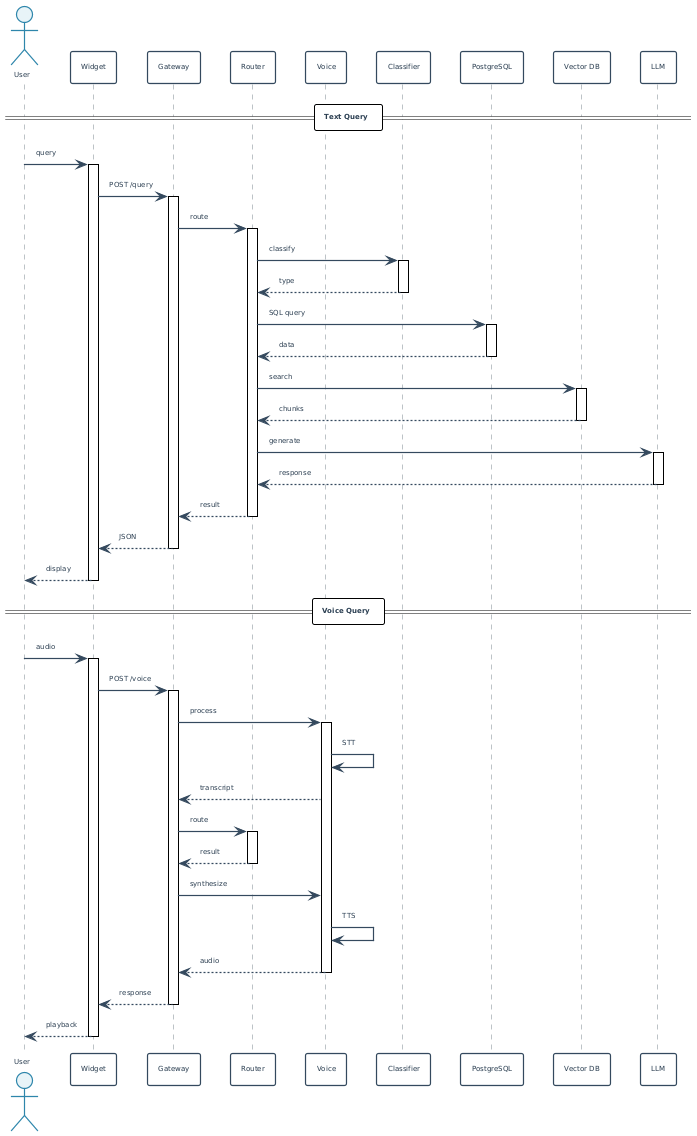
\includegraphics[width=0.95\textwidth]{diagrams/seq_query.png}
    \caption{Sequence Diagram - Multi-Modal Query Processing}
    \label{fig:seq_query}
\end{figure}

\subsubsection{Content Upload and Processing}

Figure~\ref{fig:seq_upload} shows the content upload workflow: document/URL submission, text extraction, chunking, embedding generation, and vector storage.

\begin{figure}[H]
    \centering
    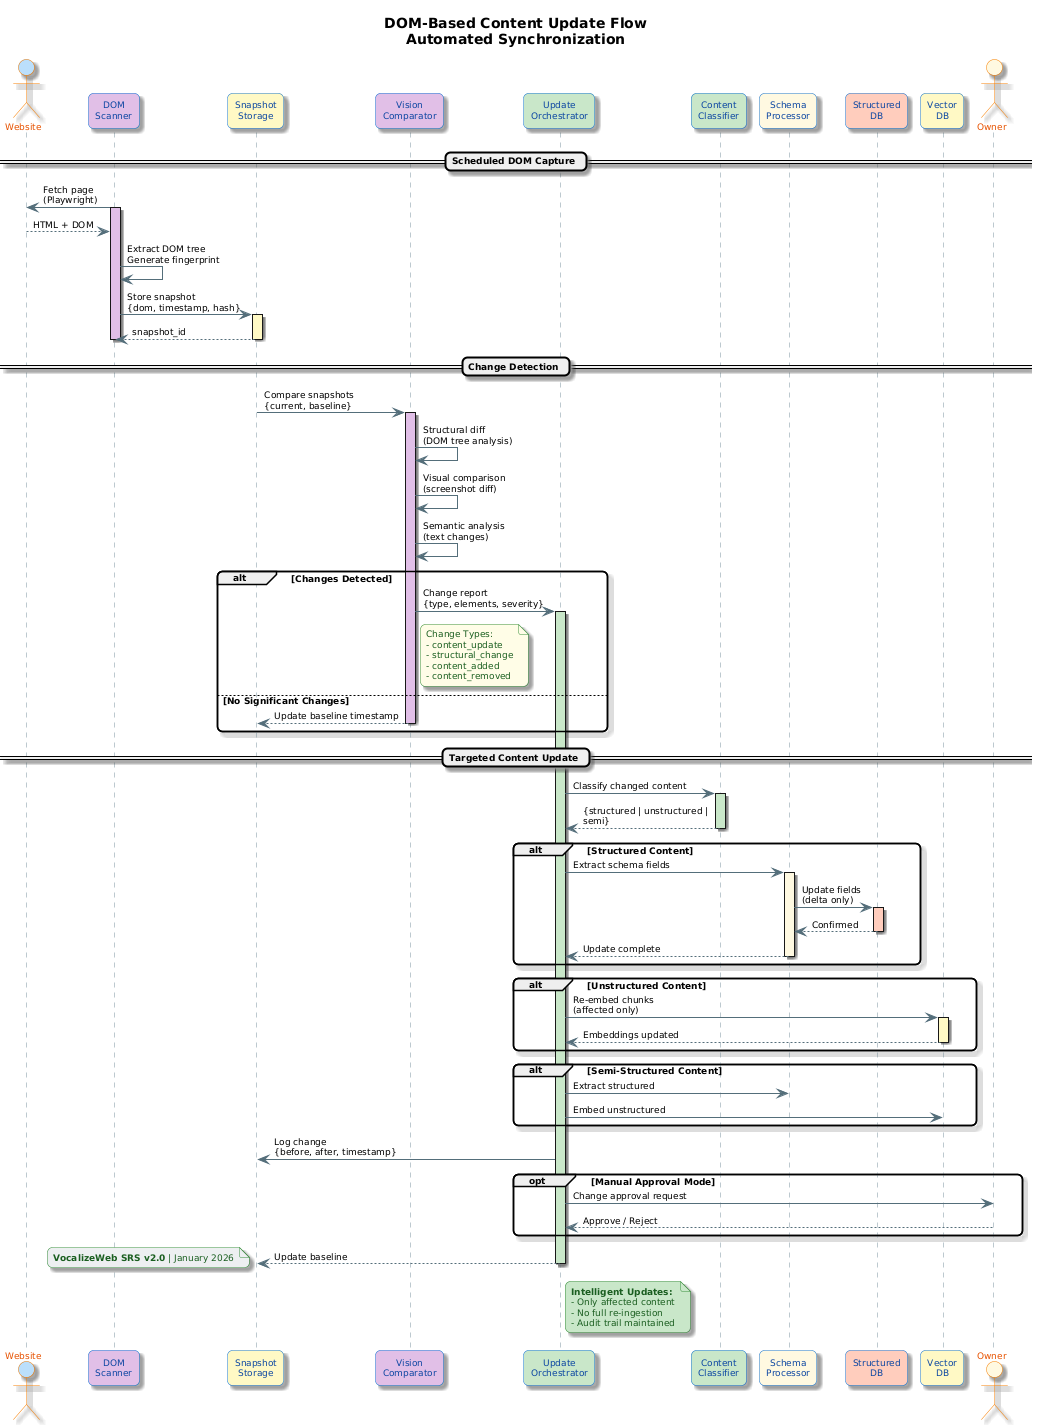
\includegraphics[width=0.95\textwidth]{diagrams/seq_upload.png}
    \caption{Sequence Diagram - Content Upload and Processing Flow}
    \label{fig:seq_upload}
\end{figure}

\section{External Interface Requirements}

\subsection{User Interfaces}

\subsubsection{Multi-Modal Widget}

The primary user interface adapts based on configured modalities:
\begin{itemize}[leftmargin=*]
    \item \textbf{Text Mode:} Floating button expands to chat panel with text input and transcript display
    \item \textbf{Voice Mode:} Floating button activates voice recording with visual states
    \item \textbf{Both Modes:} Combined interface with toggle between text and voice input
\end{itemize}

\subsubsection{Administrative Dashboard}

The dashboard provides:
\begin{itemize}[leftmargin=*]
    \item \textbf{Content Management:} View uploaded content, trigger re-ingestion, manage knowledge base
    \item \textbf{Scraping Configuration:} Configure pages for scraping, view scraping history
    \item \textbf{Feature Toggles:} Enable/disable modalities and auto-update features
    \item \textbf{Analytics:} Usage metrics, query patterns, response quality indicators
\end{itemize}

\subsection{Software Interfaces}

\subsubsection{AI Service Integrations}

\begin{itemize}[leftmargin=*]
    \item \textbf{OpenAI Whisper API:} Audio to text transcription
    \item \textbf{OpenAI Chat Completions:} Response generation with RAG context
    \item \textbf{OpenAI TTS API:} Text to speech synthesis
    \item \textbf{Embedding API:} Vector generation for semantic search
\end{itemize}

\subsubsection{Database Interfaces}

\begin{itemize}[leftmargin=*]
    \item \textbf{PostgreSQL:} Structured content, SaaS platform data via SQLAlchemy ORM
    \item \textbf{Weaviate/Redis:} Vector storage and similarity search via client libraries
\end{itemize}

\section{Constraints and Assumptions}

\subsection{Constraints}

\begin{itemize}[leftmargin=*]
    \item API usage costs for OpenAI services require optimization for profitability
    \item Web scraping frequency limited by target website terms of service
    \item Browser security restrictions limit audio processing capabilities
\end{itemize}

\subsection{Assumptions}

\begin{itemize}[leftmargin=*]
    \item Clients have rights to scrape their own website content
    \item Website structures remain relatively stable between captures
    \item Users have stable internet connectivity for real-time interaction
    \item Target websites do not employ aggressive anti-bot measures
\end{itemize}
